% Chapter 4

%%%
%\newcommand{\tabhead}[1]{\textbf{#1}}
%%%

\chapter{Optical follower servo} % Main chapter title
\label{OFS} 

In order to achieve the low-noise and accurate modulation, an active controller (servo) can modulate the waveform by means of feedback control. This feedback loop used for the Pcal is called as the Optical Follower Servo (OFS).
The OFS will be used in the KAGRA Pcal as a means to reduce the relative power noise (RPN) of the laser. We will achieve maximum sideband to carrier suppression of the modulated output waveform. 
The block diagram of the OFS is shown in Fig.~\ref{fig:OFS_diagram}. The transfer function of this diagram can be described as
\begin{equation}
\frac{AG_1}{1+AKSG_1G_2},
\end{equation}
where A is actuation factor, S is sensing factor, K is percentage of light power sampled, $G_1$ and $G_2$ are gain of feedforward and feedback.

\begin{figure}
\begin{center}
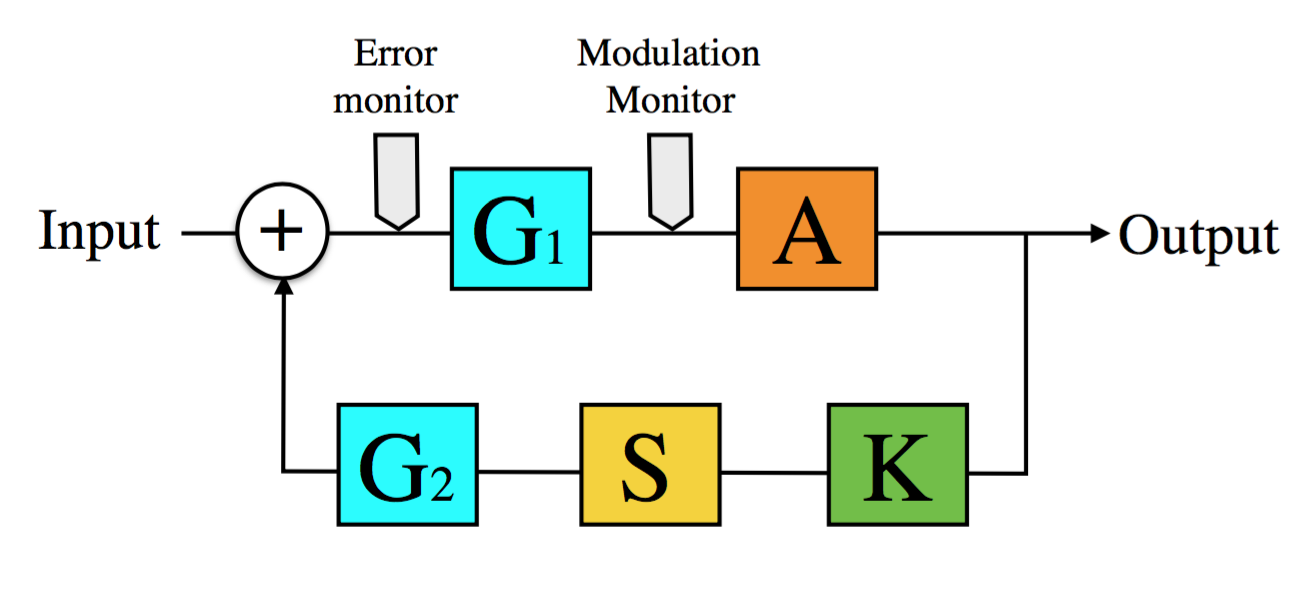
\includegraphics[width=14cm]{Figures/OFS_diagram.eps}
\caption{Diagram of feedback loop for OFS.} 
\label{fig:OFS_diagram} 
\end{center}
\end{figure}


We monitor the difference between test input and \{out1,out2,out3\} .
For monitoring the performance of OFS, we read the location of monitor point.
When we inject the signal, such as swept sine, gauss sine and hardware injection signal, we use input port.
 The estimation of the expected gain parameter is listed in Table.~\ref{tab:OFS_Gain}.

\begin{table}
\caption{Typical gain parameter of OFS. }
\label{tab:OFS_Gain}
\centering
\begin{tabular}{ ccc}
\toprule
\tabhead{} & \tabhead{Gain}& \tabhead{unit} \\
\midrule
A &  0.5 & W/V\\
$G_1$ & 10-100 & V/V(dB) \\
$G_2$ & 2 & V/V(dB) \\
KS &  0.5 & V/W \\
\bottomrule\\
\end{tabular}
\end{table}

The KS corresponds to the trans impedance gain of detector. The detail of photo detector is descrived in Sec.\ref{PD}.
According to Table.~\ref{tab:OFS_Gain}, we regard $G_2KS$ as unity. Therefore, we can simplify the transfer function as follows:
\begin{equation}
\frac{AG_1}{1+AG_1}
\end{equation}
We require the band width of OFS mach larger than operation frequency. 